\documentclass[twocolumn, fontsize=10pt]{article}
\usepackage[margin=0.70in]{geometry}
\usepackage{lipsum,mwe,abstract}
\usepackage[english]{babel} 
\usepackage{fancyhdr} % Custom headers and footers
\usepackage{multicol}
\usepackage{geometry}
\geometry{a4paper, margin=1in}
\pagestyle{fancyplain} % Makes all pages in the document conform to the custom headers and footers
\fancyhead{} 
\fancyfoot[C]{\thepage} % Page numbering for right footer
\setlength\parindent{0pt} 
\usepackage{amsmath,amsfonts,amsthm} % Math packages
\usepackage{wrapfig}
\usepackage{graphicx}
\usepackage{float}
\usepackage{subcaption}
\usepackage{comment}
\usepackage{enumitem}
\usepackage{makeidx}
\makeindex
\usepackage{cuted}
\usepackage{sectsty} % Allows customizing section commands
\usepackage{xcolor} % For colored text
\usepackage{hyperref} % Package for links
\hypersetup{
    colorlinks=true,
    linkcolor=blue,
    filecolor=magenta,      
    urlcolor=blue,
    }
\allsectionsfont{\normalfont \normalsize \scshape} % Section names in small caps and normal fonts

\addto\captionsenglish{\renewcommand{\contentsname}{Índice}}

\renewenvironment{abstract} % Change how the abstract look to remove margins
 {\small
  \begin{center}
  \bfseries Resumen \vspace{-.5em}\vspace{0pt}
  \end{center}
  \list{}{%
    \setlength{\leftmargin}{0mm}
    \setlength{\rightmargin}{\leftmargin}%
  }
  \item\relax}
 {\endlist}

 \newenvironment{englishabstract} % Abstract en inglés
 {\small
  \begin{center}
  \bfseries Abstract \vspace{-.5em}\vspace{0pt}
  \end{center}
  \list{}{%
    \setlength{\leftmargin}{0mm}
    \setlength{\rightmargin}{\leftmargin}%
  }
  \item\relax}
 {\endlist}
 
\makeatletter
\renewcommand{\maketitle}{\bgroup\setlength{\parindent}{0pt} % Change how the title looks like
\begin{flushleft}
  \begin{center}
    {\color{black} \Large Past2Polygon:  \\
    \color{black} Un enfoque basado en Machine Learning para la digitalización de mapas históricos. \\ \vspace{10pt}}
    \href{https://github.com/DanielMPMatCom/ML-Project.git}{GitHub} % Add GitHub link here
    \vspace{10pt}
  \end{center}
  \textbf{\@title}
  \@author \\ 
  \@date
\end{flushleft}\egroup
}
\makeatother

%% ------------------------------------------------------------------- 

\title{Facultad de Matemática y Computación. Universidad de La Habana.\\}

\author{
    \centering
    \begin{minipage}{\textwidth}
        \centering
        \begin{multicols}{2}
            Ariel González Gómez \\ \texttt{lenin46ariel@gmail.com} \\
            Leonardo Artiles Montero \\ \texttt{leo16am@gmail.com} \\[1em]
            Alex S. Bas Beovides \\ \texttt{abasbeovides@gmail.com} \\[1em]
            \columnbreak
            Paula Silva Lara \\ \texttt{paula.silvalara030410@gmail.com} \\[1em]
            Ricardo Cápiro Colomar \\ \texttt{rikikpiro02@gmail.com} \\[1em]
            Daniel Machado Pérez \\ \texttt{daniel.machado.0206@gmail.com}
        \end{multicols}
    \end{minipage}
}
\date{\vspace{2em}\large 30 de enero de 2025}

\begin{document}

\twocolumn[ \maketitle ]



% --------------- ABSTRACT
\begin{abstract}
En este trabajo se presenta un proceso para la digitalización y modernización de mapas antiguos, con un enfoque en la ciudad de La Habana. El objetivo es convertir estos mapas en formatos digitales modernos para facilitar su análisis y comparación con datos actuales. El proceso incluye la eliminación de ruido y etiquetas textuales mediante técnicas de procesamiento de imágenes y aprendizaje profundo. Luego, se genera un mapa de calor para identificar calles y bloques de edificios, permitiendo una segmentación precisa. Posteriormente, los bloques se vectorizan, simplifican y georreferencian, alineándolos con mapas contemporáneos. Este enfoque permite preservar y estudiar la evolución urbana de La Habana.
\end{abstract}

\begin{englishabstract}
This work presents a process for the digitization and modernization of historical maps, focusing on the city of Havana. The objective is to convert these maps into modern digital formats to facilitate their analysis and comparison with current data. The process includes noise removal and text label elimination using image processing techniques and deep learning. A heatmap is then generated to identify streets and building blocks, enabling precise segmentation. Subsequently, the blocks are vectorized, simplified, and georeferenced, aligning them with contemporary maps. This approach allows for the preservation and study of Havana's urban evolution.
\end{englishabstract}

\rule{\linewidth}{0.5pt}


% --------------- KEYWORDS
\noindent \textbf{Palabras Clave}: Digitalización, Mapas Históricos, Georreferenciación, Segmentación de Imágenes, Aprendizaje Profundo, Visión por Computadora, PaddleOCR, DBSCAN, Heatmaps, Ramer-Douglas-Peucker, Optimización Bayesiana, Shapely, CNN, Índice de Jaccard


\rule{\linewidth}{0.5pt}

% --------------- MAIN CONTENT

\tableofcontents

\rule{\linewidth}{0.5pt}
\section{Introducción}
El estudio de mapas históricos constituye una herramienta fundamental en la investigación sobre la evolución urbana, ya que permite analizar patrones de crecimiento, cambios en la infraestructura y la conservación patrimonial. En el caso de La Habana, una ciudad con una rica historia urbanística, la digitalización de mapas antiguos ofrece una oportunidad única para evaluar su transformación a lo largo del tiempo.

Los enfoques tradicionales de digitalización de mapas han recurrido a la vectorización manual o a técnicas semiautomatizadas para la detección de estructuras urbanas. Sin embargo, estos métodos presentan limitaciones en términos de escalabilidad y precisión. En este trabajo, se propone un enfoque automatizado basado en visión por computadora y aprendizaje profundo para la segmentación, extracción y georreferenciación de mapas antiguos.

El proceso comienza con el preprocesamiento de los mapas, eliminando ruido y mejorando la calidad de las imágenes mediante filtros y transformaciones. La eliminación de etiquetas textuales se lleva a cabo con PaddleOCR, con optimización adicional basada en cortes y rotaciones de la imagen para mejorar la detección. Posteriormente, se emplea una red neuronal convolucional para generar un mapa de calor que distingue entre calles y bloques de edificios.

Para la segmentación de los elementos urbanos, se utiliza un algoritmo de \textit{Flood Fill}, integrando la información del mapa de calor para mejorar la identificación de bloques urbanos. Estos bloques se convierten en polígonos vectorizados, aplicando simplificación geométrica con los algoritmos de Ramer-Douglas-Peucker (RDP) y Shapely.

Una de las innovaciones clave de este trabajo es la optimización en la identificación de polígonos atípicos mediante DBSCAN, con la selección óptima de hiperparámetros a través de optimización bayesiana. Además, se introduce un algoritmo novedoso para la comparación de polígonos topológicamente similares, basado en la normalización a área unitaria, rotaciones alineadas por pares de lados trasladados al origen y la evaluación del Índice de Jaccard o Intersection over Union (IoU). Finalmente, los mapas históricos se alinean con mapas actuales mediante georreferenciación, permitiendo su integración en plataformas SIG modernas.

Los datos fueron proporcionados por la Oficina del Historiador de la Ciudad de La Habana, y pueden ser encontrados en su \href{https://repositoriodigital.ohc.cu/s/repositoriodigital/item-set/73018}{Repositorio Digital. Colección de Planos}.

\rule{\linewidth}{0.5pt}
\section{Preprocesamiento de Imágenes}


Antes del procesamiento y análisis de los mapas, fue necesario realizar una etapa de preprocesamiento con el objetivo de mejorar la calidad de los datos y eliminar aquellos elementos que pudieran afectar el desempeño de los algoritmos de visión por computadora.

El preprocesamiento de las imágenes consistió en las siguientes tareas:

\begin{itemize}
    \item \textbf{Recorte de bordes}: Algunos mapas presentaban daños físicos como roturas o pedazos faltantes de papel, lo que generaba ruido en la aplicación de filtros de OpenCV. Se eliminaron estas áreas afectadas para mejorar la uniformidad del dataset.
    \item \textbf{Selección de datos útiles}: Se identificaron mapas en mal estado, con representaciones desproporcionadas o ilegibles debido a su antigüedad. Estos fueron descartados para evitar problemas en el análisis posterior.
    \item \textbf{Mejora de imágenes}: Algunas imágenes fueron editadas utilizando herramientas como Photoshop para optimizar su calidad. Entre las modificaciones realizadas se encuentran ajustes de color, conversión a blanco y negro y eliminación de elementos no cartográficos como carteles o anotaciones manuscritas.
\end{itemize}

Tras el proceso de filtrado y clasificación, el conjunto de datos quedó organizado de la siguiente manera:


\textbf{Datos Útiles}
\begin{itemize}
    \item \textbf{La Habana}: 30 imágenes de mapas generales de la ciudad. \ref{fig:map_nice}
    \item \textbf{Barrios}: 41 imágenes de mapas detallados de distintos barrios. \ref{fig:map_barrio}
    \item \textbf{Azules}: 50 imágenes de planos específicos de barrios de La Habana. \ref{fig:map_blue}
\end{itemize}

    \begin{figure}[H]
    \centering
    \includegraphics[width=\columnwidth]{assets/map_nice.png}
    \caption{Mapa de La Habana}
    \label{fig:map_nice}
\end{figure}

   \begin{figure}[H]
    \centering
    \includegraphics[width=\columnwidth]{assets/map_barrio.png}
    \caption{Mapa de un barrio de La Habana}
    \label{fig:map_barrio}
\end{figure}

   \begin{figure}[H]
    \centering
    \includegraphics[width=\columnwidth]{assets/map_blue.png}
    \caption{Plano azul de un barrio de La Habana}
    \label{fig:map_blue}
\end{figure}

\textbf{Datos Descartados}
\begin{itemize}
    \item \textbf{Antiguos}: 19 imágenes de mapas demasiado antiguos con poca utilidad para el análisis. \ref{fig:map_old}
    \item \textbf{Deficientes}: 90 imágenes en mal estado o con deficiencias graves. \ref{fig:map_useless}
    \item \textbf{3D}: 5 imágenes con representaciones tridimensionales que no eran compatibles con el modelo. \ref{fig:map_3D}
\end{itemize}

  \begin{figure}[H]
    \centering
    \includegraphics[width=\columnwidth]{assets/map_old.png}
    \caption{Mapa antiguo de La Habana}
    \label{fig:map_old}
\end{figure}

  \begin{figure}[H]
    \centering
    \includegraphics[width=\columnwidth]{assets/map_useless.png}
    \caption{Mapa de la Playa Santa María, La HabanaMapa 3D de La Habana}
    \label{fig:map_useless}
\end{figure}

  \begin{figure}[H]
    \centering
    \includegraphics[width=\columnwidth]{assets/map_3D.png}
    \caption{Mapa 3D de La Habana}
    \label{fig:map_3D}
\end{figure}

En la Figura \ref{fig:before_after} se muestra un ejemplo de una imagen antes y después de preprocesarla


  \begin{figure}[H]
    \centering
    \includegraphics[width=\columnwidth]{assets/before_after.jpg}
    \caption{Mapa antes y después de preprocesar}
    \label{fig:before_after}
\end{figure}

\rule{\linewidth}{0.5pt}
\section{Extracción y Eliminación de Etiquetas (\textit{Labels })}

Los mapas históricos contienen etiquetas textuales que identifican calles y lugares. Sin embargo, estas etiquetas pueden introducir ruido en los sistemas automatizados de análisis de mapas, ya que los trazos de las letras pueden ser malinterpretados como líneas que representan polígonos. La detección y eliminación de estas etiquetas es un paso crucial en el preprocesamiento para mejorar la interpretación automatizada de mapas históricos.

\begin{figure}[H]
    \centering
    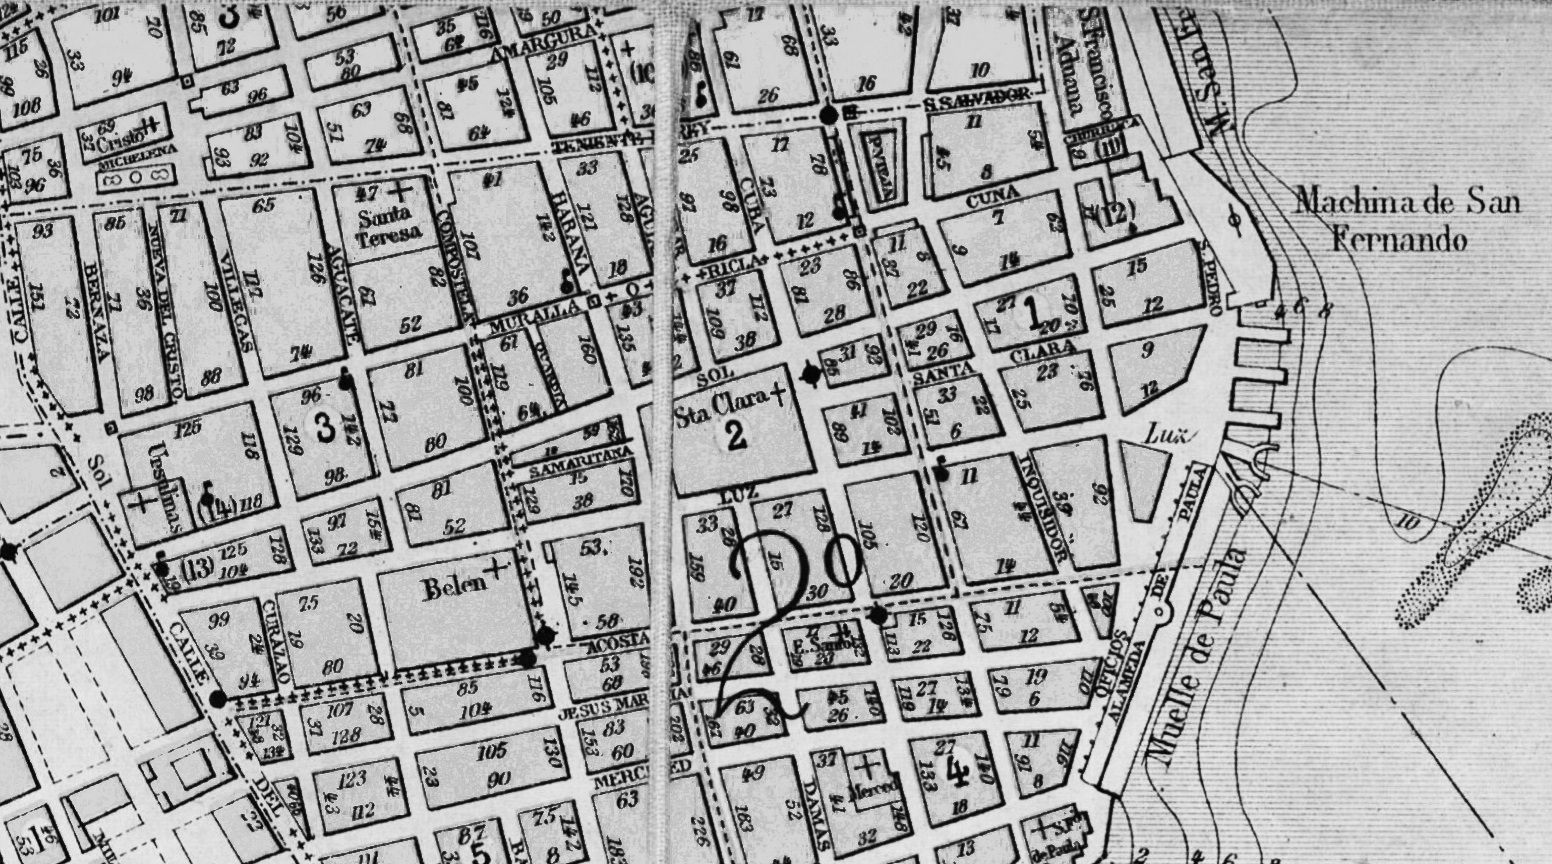
\includegraphics[width=\columnwidth]{assets/tiny_map.jpg}
    \caption{Imagen preprocesada.}
    \label{fig:tiny_map}
\end{figure}

\subsection{Detección de Texto con PP-OCR}
PP-OCR \cite{ocr}, es un sistema OCR ultraligero diseñado para eficiencia y precisión. Este modelo emplea \textit{Differentiable Binarization} (DB) \cite{diffbin} para una segmentación robusta del texto y está basado en MobileNetV3 \cite{mobilenet}, lo que optimiza la velocidad de procesamiento y minimiza el consumo de memoria. Su entrenamiento se ha realizado en un conjunto diverso de 97,000 imágenes, incluyendo:
\begin{itemize}
    \item 68,000 imágenes reales obtenidas de conjuntos de datos públicos y búsquedas en Baidu.
    \item 29,000 imágenes sintéticas con diversos estilos y orientaciones de texto.
\end{itemize}

Los conjuntos de datos empleados incluyen:
\begin{itemize}
    \item \textbf{LSVT}: Texto en vistas urbanas a gran escala.
    \item \textbf{RCTW-17}: Texto en documentos escaneados.
    \item \textbf{MTWI 2018}: Imágenes con texto mixto.
    \item \textbf{CASIA-10K}: Texto en documentos oficiales.
    \item \textbf{SROIE}: OCR en recibos y facturas.
    \item \textbf{MLT 2019}: Detección de texto en múltiples idiomas.
    \item \textbf{MSRA-TD500}: Señales de tráfico y carteles.
    \item \textbf{CCPD 2019}: Reconocimiento de matrículas vehiculares.
\end{itemize}

\begin{figure}[H]
    \centering
    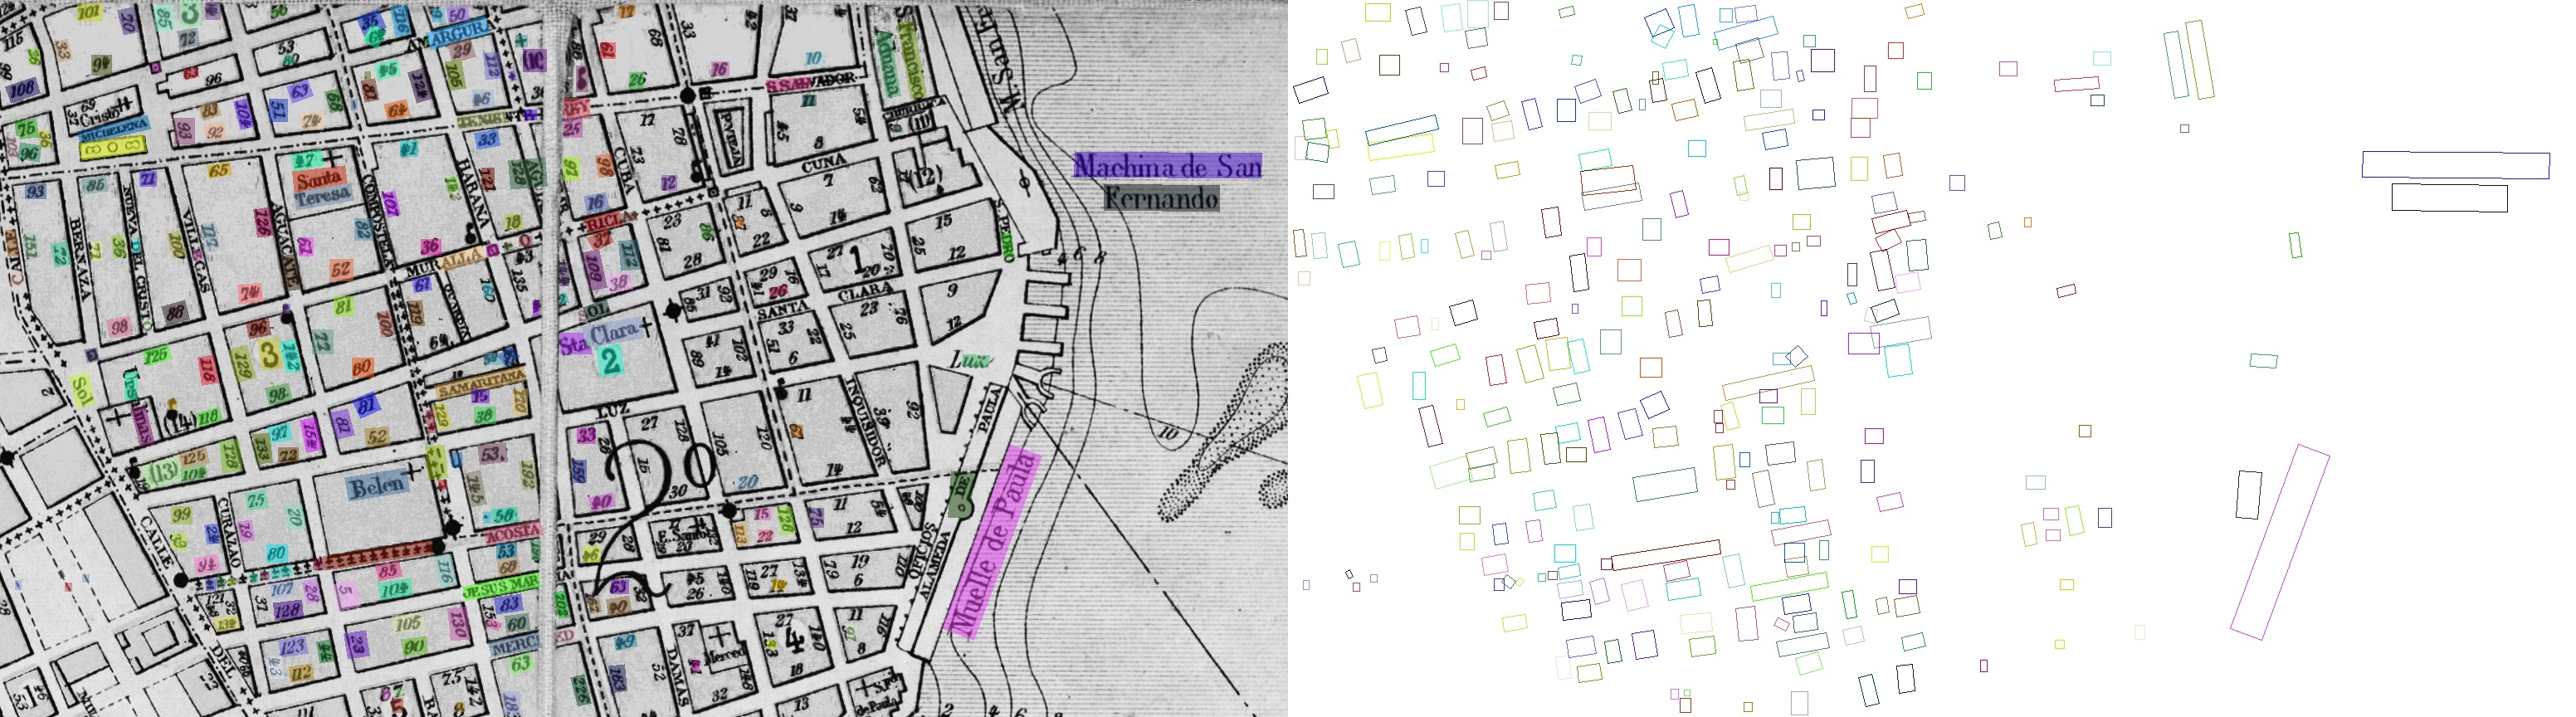
\includegraphics[width=\columnwidth]{assets/tiny_map_colored_labels.jpg}
    \caption{Imagen con etiquetas detectadas.}
    \label{fig:tiny_map_colored_labels}
\end{figure}

\subsection{Manejo de Imágenes de Mapas Históricos de Gran Tamaño}
Los mapas históricos suelen tener alta resolución, lo que plantea desafíos en la detección de texto con PP-OCR debido a su tamaño de entrada fijo. El redimensionamiento automático de imágenes grandes puede comprometer la resolución y afectar la detección de texto pequeño. Para abordar este problema, la imagen se segmenta en regiones más pequeñas antes del procesamiento, permitiendo detectar el texto con mayor precisión. Posteriormente, los polígonos de texto detectados se mapean a sus coordenadas originales en la imagen completa.

\subsection{Eliminación de Texto con Agrupamiento K-Means}
Después de detectar el texto, su eliminación implica reemplazar los píxeles correspondientes con el color del fondo circundante. Métodos como la moda o el promedio de color no resultan efectivos debido a la variabilidad cromática del fondo. Por ello, se utiliza el algoritmo de agrupamiento K-Means para identificar el color predominante dentro del polígono de texto. El procedimiento es el siguiente:
\begin{itemize}
    \item Se agrupan los colores dentro del polígono en 3 \textit{clusters}.
    \item Se selecciona el \textit{cluster} dominante como color representativo del fondo.
    \item Los píxeles del texto se reemplazan por este color, integrando visualmente el área editada con el resto de la imagen.
\end{itemize}

Este método ha demostrado ser efectivo sin requerir ajustes adicionales del hiperparámetro \textbf{n\_clusters}.

\begin{figure}[H]
    \centering
    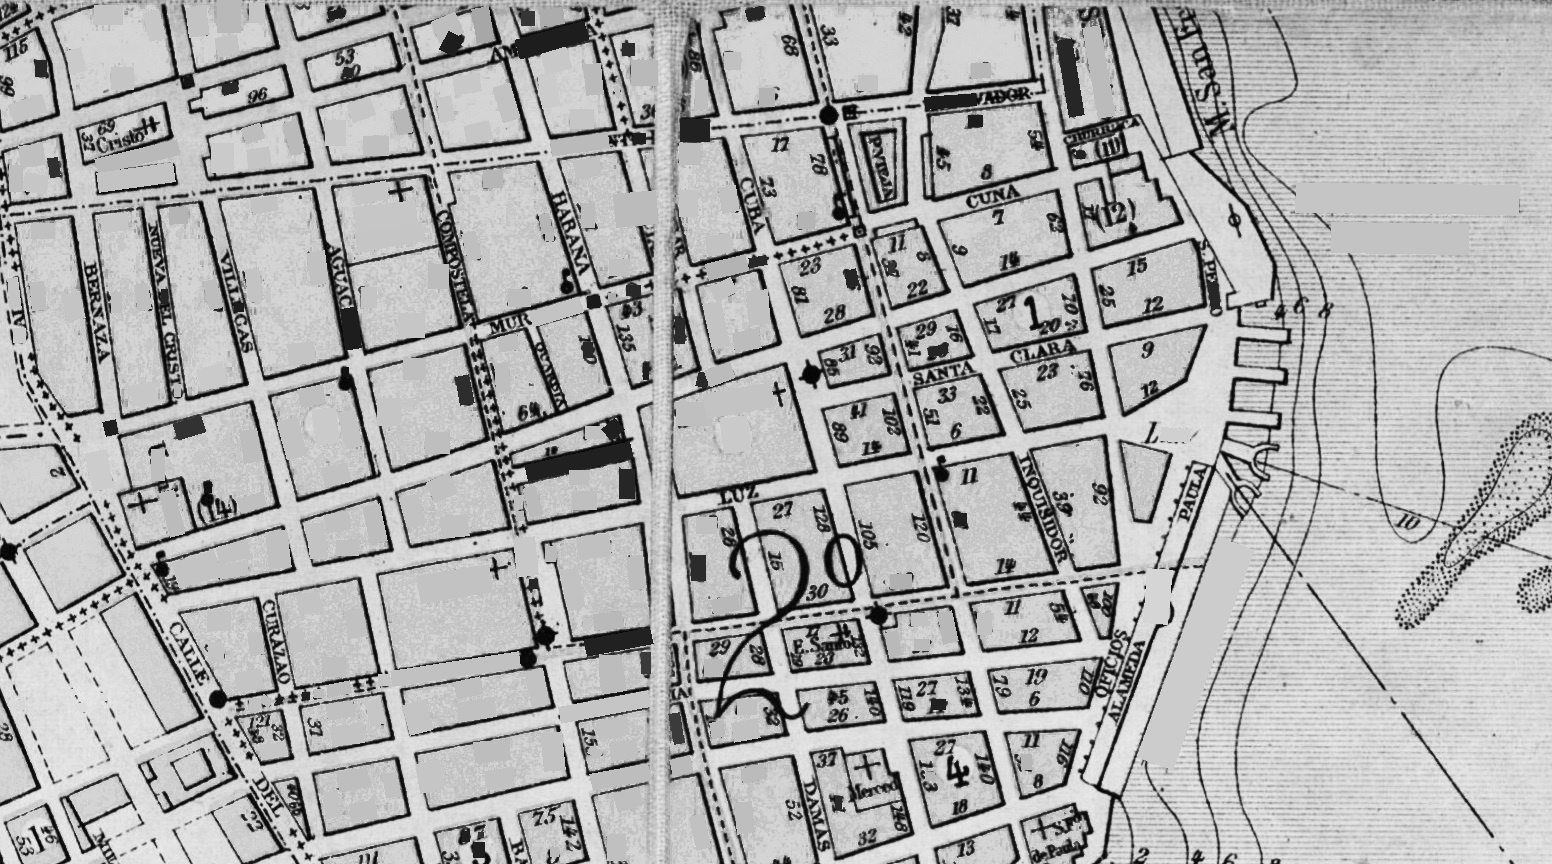
\includegraphics[width=\columnwidth]{assets/tiny_map_labelless.jpg}
    \caption{Imagen con etiquetas eliminadas.}
    \label{fig:tiny_map_labelless}
\end{figure}

\rule{\linewidth}{0.5pt}
\section{Generación de \textit{Heatmaps} de Calles}

Se entrenó un modelo basado en redes neuronales convolucionales (CNN) para la detección de calles en mapas antiguos. El objetivo es generar un mapa de calor que permita identificar las regiones correspondientes a calles y diferenciarlas de bloques de casas. Este proceso es un paso fundamental para la posterior selección de los bloques tras la segmentación.

\subsection{Creación del \textit{dataset}}

Para entrenar el modelo, se construyó un \textit{dataset} a partir de recortes de mapas. Se intentó también generar un \textit{dataset} sintético, pero este enfoque no resultó efectivo, ya que las imágenes generadas no lograban capturar la variabilidad y complejidad de los mapas reales, lo que llevó a un desempeño inferior en la detección de calles. Las imágenes fueron clasificadas en cuatro categorías \ref{fig:dataset}:

\begin{itemize}
    \item \textbf{Intersecciones de calles:} aproximadamente 1400 imágenes.
    \item \textbf{Calles (segmentos entre intersecciones):} 1500 imágenes.
    \item \textbf{Partes del mapa que no son ni calles ni intersecciones:} 1500 imágenes.
    \item \textbf{Recortes aleatorios de los mapas:} cantidad variable.
\end{itemize}

\begin{figure}[H]
    \centering
    \includegraphics[width=\columnwidth]{assets/dataset.png}
    \caption{Ejemplos de imágenes del \textit{dataset}.}
    \label{fig:dataset}
\end{figure}


Para mejorar la capacidad de generalización del modelo, se realizó data augmentation sobre la categoría de intersecciones de calles. En particular, cada imagen se rotó en tres ángulos diferentes (90°, 180° y 270°), cuadruplicando así el número de muestras en esta clase.

\subsection{Arquitectura del Modelo}

En la Figura \ref{fig:arch} se muestra un esquema gráfico de la arquitectura de la CNN utilizada para la detección de calles:

\begin{figure*}[h]
    \centering
    \includegraphics[width=0.8\textwidth]{assets/arch2.png}
    \caption{Esquema de la arquitectura de la CNN utilizada.}
    \label{fig:arch}
\end{figure*}

El modelo utilizado es una CNN con la siguiente configuración:

\begin{itemize}
    \item \textbf{Capas convolucionales:} Cuatro capas convolucionales con 32, 64, 128 y 256 filtros respectivamente, con kernel de tamaño $3\times3$ y \textit{padding} de 1.
    \item \textbf{Normalización y activación:} Se emplea \textit{Batch Normalization} después de cada capa convolucional y ReLU como función de activación.
    \item \textbf{Regularización:} Se utiliza una capa de \textit{dropout} con una tasa del 50\% para evitar el sobreajuste.
    \item \textbf{\textit{Pooling}:} Se aplica \textit{max pooling} con un tamaño de ventana $2\times2$ y \textit{stride} de 2, reduciendo progresivamente la dimensionalidad espacial de las características extraídas.
    \item \textbf{Clasificador:} Dos capas completamente conectadas, una con 512 neuronas y otra de salida con 2 neuronas para la clasificación binaria (calles vs. no calles).
\end{itemize}

\subsection{Proceso de Entrenamiento}
Se empleó la función de pérdida de entropía cruzada y el optimizador AdamW con una tasa de aprendizaje ajustable mediante un \textit{scheduler} que reducía la tasa si la pérdida de validación dejaba de mejorar.

La base de datos se dividió en 80\% para entrenamiento y 20\% para validación. Se utilizó un tamaño de batch de 32 y se entrenó por 10 épocas.

\subsection{Resultados}
Durante el entrenamiento, se observó un comportamiento inusual en las primeras épocas: la pérdida en el conjunto de validación era menor que la pérdida en el conjunto de entrenamiento, y el \textit{accuracy} de validación también era mayor que el de entrenamiento. Este fenómeno puede deberse a varios factores:

\begin{itemize}
    \item \textbf{Regularización efectiva:} Es posible que el modelo generalizara bien desde el principio debido al uso de \textit{Batch Normalization} y \textit{Dropout}, lo que impide un sobreajuste rápido a los datos de entrenamiento.
    \item \textbf{Efecto del data augmentation:} Como el conjunto de entrenamiento incluye imágenes con transformaciones adicionales, esto puede haber aumentado su complejidad inicial en comparación con las imágenes del conjunto de validación, que no sufrieron las mismas alteraciones.
\end{itemize}

A medida que avanzaron las épocas, esta diferencia se redujo y el modelo terminó mostrando una tendencia más esperada, con la pérdida de entrenamiento disminuyendo más rápidamente \ref{fig:loss} y el \textit{accuracy} de entrenamiento alcanzando valores superiores a los de validación. \ref{fig:acc}

\begin{figure}[H]
    \centering
    \includegraphics[width=\columnwidth]{assets/loss.png}
    \caption{Gráfica de la función de pérdida.}
    \label{fig:loss}
\end{figure}

\begin{figure}[H]
    \centering
    \includegraphics[width=\columnwidth]{assets/acc.png}
    \caption{Gráfica de la función de \textit{accuracy}.}
    \label{fig:acc}
\end{figure}

Se probaron diferentes enfoques para el entrenamiento del modelo. El mejor desempeño se obtuvo cuando se entrenó el modelo exclusivamente con la categoría de intersecciones de calles, aplicando data augmentation mediante rotaciones. Este enfoque permitió mejorar significativamente la capacidad del modelo para reconocer patrones en mapas antiguos y distinguir calles de bloques de casas.

\subsection{Generación del \textit{Heatmap}}
Para generar un mapa de calor que permita identificar las zonas correspondientes a calles en los mapas antiguos, se utilizó un enfoque basado en una ventana deslizante sobre la imagen. Se aplicó el modelo entrenado a pequeñas secciones de la imagen original, obteniendo una probabilidad de presencia de calles en cada región. Los resultados se combinaron en un mapa de calor normalizado para representar gráficamente las zonas con mayor probabilidad de ser calles.

Además del enfoque basado en la ventana deslizante, se experimentó con técnicas como Grad-CAM y cuadriculado para visualizar la relevancia de las activaciones del modelo. Sin embargo, estos métodos no ofrecieron resultados tan precisos como el enfoque de ventana deslizante, por lo que se optó por este último en la generación final del \textit{heatmap}.


\begin{figure}[H]
    \centering
    \includegraphics[width=\columnwidth]{assets/heatmap2.png}
    \caption{Ejemplo de \textit{heatmap} aprendido.}
    \label{fig:heatmap2}
\end{figure}

\begin{figure}[H]
    \centering
    \includegraphics[width=\columnwidth]{assets/heatmap1.png}
    \caption{Ejemplo de \textit{heatmap} aprendido.}
    \label{fig:heatmap1}
\end{figure}

\subsection{Evaluación}

La evaluaci\'on de esta parte se llev\'o a cabo 
mediante un proceso comparativo que involucr\'o la 
generaci\'on de un conjunto de datos de referencia 
(\textit{ground truth}, Figura \ref{fig:gt}) a partir de anotaciones 
manuales y la evaluaci\'on de tres modelos entrenados 
con diferentes estrategias. 

\begin{figure}[H]
    \centering
    \includegraphics[width=\columnwidth]{assets/GT.png}
    \caption{Segmentaci\'on anotada manualmente.}
    \label{fig:gt}
\end{figure}

Se evaluaron los siguinete tres modelos para la generaci\'on del \textit{heatmap}:
\begin{enumerate}
    \item \textbf{Modelo Manual:} Entrenado con datos etiquetados manualmente, en el que se definieron dos clases: \textit{intersecciones+calles} y \textit{no intersecciones ni calles}.
    \item \textbf{Modelo con Intersecciones y Recortes Aleatorios:} Se emple\'o un conjunto de datos que conten\'ia instancias de intersecciones junto con recortes aleatorios, con el fin de incrementar la diversidad del entrenamiento.
    \item \textbf{Modelo Sint\'etico:} Entrenado con datos generados totalmente de forma sint\'etica, que simulaban las caracter\'isticas de intersecciones y calles.
\end{enumerate}

Cada uno de estos modelos fue evaluado en seis im\'agenes seleccionadas, y, adicionalmente, se prob\'o la versi\'on \textit{labelless} (sin etiquetas) para analizar el comportamiento en ausencia de anotaciones. La comparaci\'on se efectu\'o mediante tres m\'etricas de evaluaci\'on no binarias, las cuales se describen a continuaci\'on:

\begin{itemize}
    \item \textbf{AUC (\textit{Area Under the ROC Curve}):} \cite{auc} Mide la capacidad del modelo para discriminar entre las dos clases. Un valor de AUC cercano a 1 indica una excelente discriminaci\'on, mientras que valores cercanos a 0.5 reflejan un desempe\~no aleatorio.
    \item \textbf{Precisi\'on Promedio:} \cite{precission} Calcula la media de la precisi\'on obtenida en diferentes niveles de \textit{recall}, ofreciendo una medida global del equilibrio entre la exactitud y la capacidad de recuperar instancias relevantes.
    \item \textbf{\textit{Brier Score}:} \cite{brier} Eval\'ua la exactitud de las probabilidades pronosticadas. Se define como el promedio del error cuadr\'atico entre la probabilidad predicha y la etiqueta real, donde valores menores indican una mejor calibraci\'on del modelo.
\end{itemize}

Las Figuras~\ref{fig:auc1}, \ref{fig:prec1} y \ref{fig:brier1} 
presentan la comparaci\'on de estas m\'etricas 
entre los distintos modelos, considerando tanto 
la versi\'on con extracci\'on de texto como la 
sin ella. Adicionalmente, las Figuras~\ref{fig:auc2}, 
\ref{fig:prec2} y \ref{fig:brier2} muestran la 
distribuci\'on de cada m\'etrica por modelo, 
permitiendo evaluar la variabilidad y consistencia del 
desempe\~no.


\begin{figure}[H]
    \centering
    \includegraphics[width=\columnwidth]{assets/auc.png}
    \caption{Comparación del \textit{AUC} entre los distintos modelos, sin y con extracción de texto.}
    \label{fig:auc1}
\end{figure}
\begin{figure}[H]
    \centering
    \includegraphics[width=\columnwidth]{assets/prec.png}
    \caption{Comparación del \textit{promedio de la precisión} entre los distintos modelos, sin y con extracción de texto.}
    \label{fig:prec1}
\end{figure}
\begin{figure}[H]
    \centering
    \includegraphics[width=\columnwidth]{assets/brier.png}
    \caption{Comparación del \textit{Brier Score} entre los distintos modelos, sin y con extracción de texto.}
    \label{fig:brier1}
\end{figure}
\begin{figure}[H]
    \centering
    \includegraphics[width=\columnwidth]{assets/aucbox.png}
    \caption{Distribución del \textit{AUC} por modelo.}
    \label{fig:auc2}
\end{figure}
\begin{figure}[H]
    \centering
    \includegraphics[width=\columnwidth]{assets/precbox.png}
    \caption{Distribución del \textit{promedio de la precisión} por modelo.}
    \label{fig:prec2}
\end{figure}
\begin{figure}[H]
    \centering
    \includegraphics[width=\columnwidth]{assets/bierbox.png}
    \caption{Distribución del \textit{Brier Score} por modelo.}
    \label{fig:brier2}
\end{figure}


Los resultados indicaron que el modelo 
entrenado con datos etiquetados 
manualmente alcanz\'o un desempeño superior, 
reflejado en un AUC mayor, un \textit{Brier Score} 
menor y una precisi\'on promedio m\'as alta, en 
comparaci\'on con el modelo sint\'etico y el modelo 
basado en intersecciones con recortes aleatorios. 
La versi\'on labelless, aunque mostr\'o ciertos 
desaf\'ios en la generaci\'on del \textit{heatmap}, 
proporcion\'o resultados comparables en t\'erminos de 
consistencia espacial. La matriz de confusión de dicho modelo se muestra en la Figura \ref{fig:conf_matr}.

\begin{figure}[H]
    \centering
    \includegraphics[width=\columnwidth]{assets/conf_matr.png}
    \caption{Matriz de Confusión de la CNN entrenada con datos etiquetados manualmente.}
    \label{fig:conf_matr}
\end{figure}

Las tablas de los resultados de las métricas aplicadas pueden ser consultadas en los Anexos.


\rule{\linewidth}{0.5pt}
\section{Segmentación de Imágenes}

En esta fase del proyecto, se aborda la segmentación de las imágenes con el objetivo de identificar y aislar componentes conexas cromáticamente similares. Este proceso es crucial para la posterior vectorización de bloques de edificios y generación de puntos de control. La segmentación se realiza sobre las imágenes obtenidas de la fase de eliminación de etiquetas, generando como resultado un conjunto de máscaras binarias que representan los contornos de las componentes identificadas, además de información asociada a cada componente.

\subsection{Metodología}
La segmentación se lleva a cabo mediante un algoritmo de \textit{Flood Fill}  \cite{floodfill} modificado, similar al funcionamiento de la herramienta "cubo de pintura" en programas de edición de imágenes. Este algoritmo se aplica de forma iterativa a cada píxel no visitado, explorando sus vecinos y agrupando aquellos que comparten características de color similares.

\subsubsection{Algoritmo de Flood Fill Modificado}
El algoritmo de \textit{Flood Fill} se adapta para la segmentación considerando la similitud cromática entre píxeles. El proceso se describe como sigue:

\begin{enumerate}
    \item Se inicia con un píxel no visitado como semilla.
    \item Se expande a los píxeles vecinos, incluyendo los píxeles adyacentes por los lados, y opcionalmente por las diagonales, verificando si la diferencia de color con respecto al píxel inicial (o al último píxel visitado) es menor que un umbral ($\textit{k}$).
    \item Si la diferencia de color es menor que $\textit{k}$, el píxel se agrega a la componente actual y se marca como visitado.
    \item El proceso se repite iterativamente hasta que no queden píxeles conectados que cumplan con el umbral de diferencia de color.
    \item Se obtienen los pixeles que forman la componente segmentada.
\end{enumerate}

La diferencia de color entre dos píxeles se calcula mediante una distancia, la cual puede ser la diferencia absoluta de los valores RGB, o la distancia Euclídea en el espacio de color RGB. Sean $c_1 = (r_1, g_1, b_1)$ y $c_2 = (r_2, g_2, b_2)$ los colores de dos píxeles, la diferencia de color se calcula como:

\begin{itemize}
    \item Distancia Absoluta: 
     \[\text{diff}(c_1, c_2) = |r_1 - r_2| + |g_1 - g_2| + |b_1 - b_2|\] 
    \item Distancia Euclídea:
    \[\text{diff}(c_1, c_2) = \sqrt{(r_1 - r_2)^2 + (g_1 - g_2)^2 + (b_1 - b_2)^2}\]
\end{itemize}

Una vez completado el proceso de segmentación de una componente, se calcula el \textit{bounding box} que la engloba, almacenando su ubicación (píxel de la esquina superior izquierda) y dimensiones (ancho y alto).

\subsubsection{Clasificación de Componentes}
Tras segmentar las imágenes en componentes, se realiza una clasificación para distinguir entre componentes que representan bloques de edificios y aquellas que no. Esta clasificación se basa en el análisis de un mapa de calor previamente generado en la fase anterior. Para cada componente, se calcula el promedio de las probabilidades de ser parte de un bloque de edificios de todos sus pixeles.

Si el promedio de probabilidades supera un umbral determinado, la componente se considera un bloque de edificios; de lo contrario, se clasifica como un componente no relacionado. Además, se descartan componentes de tamaño inferior a un umbral mínimo, ya que se consideran ruido o texto en la imagen.

\subsection{Hiperparámetros}
La precisión de la segmentación depende de la configuración de varios hiperparámetros, los cuales se ajustan de forma empírica:



\begin{itemize}
    \item \textit{k}: Umbral de similitud de color. Determina la tolerancia en la diferencia de color para considerar dos píxeles como parte de la misma componente.
    \item \textit{use8Way}: Booleano que activa o desactiva el uso de los 8 vecinos en la busqueda de componentes conexas. Si es falso, solo los 4 vecinos ortogonales.
    \item \textit{euclidif}: Booleano que activa o desactiva el uso de la distancia euclídea en vez de la absoluta para calcular la diferencia de color.
    \item \textit{adj}: Booleano que indica si la comparación se hace con respecto al ultimo pixel visitado o el inicial.
    \item \textit{minComponentSize}: Tamaño mínimo (en número de píxeles) para que una componente sea considerada válida.
    \item \textit{buildingBlockTreshold}: Umbral de probabilidad promedio para clasificar una componente como un bloque de edificios.
\end{itemize}

\subsection{Salidas}
Como resultado de esta fase, se obtienen los siguientes archivos por cada imagen procesada:

\begin{itemize}
    \item Máscaras binarias: Imágenes en formato JPG que contienen las máscaras binarias de cada componente identificada, separadas en dos carpetas: una para componentes clasificadas como bloques de edificios y otra para las no relacionadas.
    \item Imagen de segmentación: Una imagen en formato JPG que visualiza la segmentación, donde cada componente se muestra con un color aleatorio.
        \item Imagen de componentes de edificios: Una imagen en formato JPG que visualiza las componentes clasificadas como bloques de edificios.
    \item Archivo de información: Un archivo en formato JSON con información detallada sobre cada componente extraída, incluyendo su bounding box (coordenadas de la esquina superior izquierda, ancho y alto) y la probabilidad de que sea un bloque de edificios.
\end{itemize}

Estos resultados constituyen la entrada para las siguientes etapas del proyecto, en particular, la vectorización de bloques de edificios.

\begin{figure}[H]
    \centering
    \includegraphics[width=\columnwidth]{assets/segmentation.jpg}
    \caption{Mapa preprocesado (arriba), Segmentación coloreada (medio), Máscara de bloques de edificios (abajo).}
    \label{fig:segmentation}
\end{figure}

\begin{figure}[H]
    \centering
    \includegraphics[width=\columnwidth]{assets/segmentation2.jpg}
    \caption{Mapa preprocesado (arriba), Segmentación coloreada (medio), Máscara de bloques de edificios (abajo).}
    \label{fig:segmentation2}
\end{figure}

\begin{figure}[H]
    \centering
    \includegraphics[width=\columnwidth]{assets/blocksvsnoblocks.jpg}
    \caption{Componentes clasificadas como bloques de edificios (arriba), Resto de componentes (abajo).}
    \label{fig:blocksvsnoblocks}
\end{figure}

\subsection{Evaluación}

Como la etapa de segmentaci\'on produce un mapa binario que distingue las \'areas de inter\'es (por ejemplo, manzanas o bloques) del fondo, se emplearon m\'etricas de clasificaci\'on 
binaria para evaluar su calidad. 
En concreto, se utilizaron:

\begin{itemize}
    \item \textbf{Dice Score}: \cite{dice} Mide la superposici\'on entre el mapa predicho y el mapa de referencia, con valores cercanos a 1 indicando una mayor similitud.
    \item \textbf{IoU (Intersection over Union)}: \cite{iou} Calcula la proporci\'on de la intersecci\'on entre la regi\'on segmentada y la regi\'on real frente a su uni\'on total. Valores m\'as altos reflejan mayor precisi\'on en la delimitaci\'on de la regi\'on.
    \item \textbf{Precisi\'on}: Mide cu\'antos de los p\'ixeles clasificados como positivos (manzanas) son realmente positivos, ofreciendo una perspectiva sobre la exactitud de la detecci\'on.
\end{itemize}

En esta fase se compararon dos configuraciones: una en la que se manten\'ian las etiquetas o texto dentro de la imagen (\textit{Normal}), y otra en la que se hab\'ian eliminado dichos elementos (\textit{Labeless}). Los resultados, ilustrados en las Figuras~\ref{fig:dice}, \ref{fig:iou} y \ref{fig:precision}, muestran que la versi\'on \textit{Labeless} presenta valores superiores de \textit{Dice}, \textit{IoU} y \textit{Precisi\'on}, lo cual indica una mejor segmentaci\'on. Esto sugiere que la eliminaci\'on de etiquetas textuales contribuy\'o a reducir el ruido en la imagen y, en consecuencia, a mejorar la detecci\'on de las \'areas de inter\'es.

\begin{figure}[H]
    \centering
    \includegraphics[width=\columnwidth]{assets/dice.png}
    \caption{Comparaci\'on del \textit{Dice Score} entre im\'agenes con y sin texto.}
    \label{fig:dice}
\end{figure}

\begin{figure}[H]
    \centering
    \includegraphics[width=\columnwidth]{assets/iou.png}
    \caption{Comparaci\'on del \textit{IoU} entre im\'agenes con y sin texto.}
    \label{fig:iou}
\end{figure}

\begin{figure}[H]
    \centering
    \includegraphics[width=\columnwidth]{assets/precision.png}
    \caption{Comparaci\'on de la \textit{precisi\'on} entre im\'agenes con y sin texto.}
    \label{fig:precision}
\end{figure}

La notable diferencia de desempe\~no entre ambas configuraciones refuerza la hip\'otesis de que la presencia de etiquetas o texto en las im\'agenes puede interferir en la etapa de segmentaci\'on, generando falsos positivos o confundiendo la red. En cambio, al retirar estos elementos, el modelo se centr\'o en la morfolog\'ia de las manzanas y logr\'o una segmentaci\'on m\'as fiel a la estructura urbana real.


\rule{\linewidth}{0.5pt}
\section{Vectorización de Polígonos}


La vectorización constituyó un paso esencial en el procesamiento de los datos, permitiendo la conversión de estructuras raster a representaciones geométricas vectoriales. Este proceso comenzó con la recepción de imágenes que contenían los polígonos de interés, junto con la información complementaria almacenada en el archivo \texttt{components\_info.json}. La combinación de estas fuentes de datos permitió garantizar una correspondencia precisa entre los elementos geoespaciales y sus atributos asociados.\\

Inicialmente, cada imagen fue procesada para su preparación antes de la vectorización. El procedimiento incluyó la conversión a escala de grises y la binarización mediante la aplicación de un umbral fijo. \\

\begin{figure}[H]
    \centering
    \includegraphics[width=\columnwidth]{assets/polygons.jpg}
    \caption{Ejemplo de imágenes a vectorizar.}
    \label{fig:polygons}
\end{figure}


Posteriormente, la imagen binarizada fue almacenada en formato GeoTIFF con la proyección espacial EPSG:4326. Este formato permitió conservar las referencias espaciales y facilitó la integración con herramientas SIG, como QGIS \cite{qgis}, para su visualización y análisis posterior.

\begin{figure}[H]
    \centering
    \includegraphics[width=\columnwidth]{assets/qgis.png}
    \caption{Ejemplo de uso de QGIS.}
    \label{fig:qgis}
\end{figure}

\subsection{Vectorización del Raster}

Una vez obtenida la imagen binarizada, se empleó el módulo \texttt{gdal\_polygonize.py} para la vectorización. Este proceso generó un conjunto de polígonos almacenados en formato Shapefile. En esta etapa, se aplicó un filtrado para seleccionar el polígono principal basado en su \textit{área} como criterio de prioridad. Este filtrado permitió eliminar elementos espurios y garantizar que la información extraída fuera relevante para el análisis.

\begin{figure}[H]
    \centering
    \includegraphics[width=\columnwidth]{assets/vectorized.png}
    \caption{Resultado de vectorizar el polígono.}
    \label{fig:vectorized}
\end{figure}

\subsection{Simplificación de Polígonos}

Para reducir la complejidad geométrica de los polígonos vectorizados, se implementó una fase de simplificación mediante dos métodos distintos: el algoritmo de Ramer-Douglas-Peucker (RDP) \cite{rdp} y el método de simplificación de Shapely \cite{shapely}. 

\begin{figure}[H]
    \centering
    \includegraphics[width=\columnwidth]{assets/rdp.png}
    \caption{Ejemplo ilustrativo del proceso de simplificación de polígonos con RDP.}
    \label{fig:rdp}
\end{figure}

\begin{figure}[H]
    \centering
    \includegraphics[width=\columnwidth]{assets/simplified.png}
    \caption{Resultado de simplificar la geometría del polígono.}
    \label{fig:simplified}
\end{figure}

Se realizaron comparaciones entre ambos enfoques para evaluar su efectividad en la preservación de la estructura original del polígono mientras se minimizaba la cantidad de vértices. Las principales diferencias en cuanto a los resultados se sustentan en lo siguiente:

\begin{itemize}
    \item \textbf{rdp:} Implementa únicamente Douglas-Peucker, lo que lo hace específico para simplificación basada en la distancia.

\item \textbf{shapely:} Es más general, basado en un algoritmo de topología-preservación y puede ser más preciso en algunos casos.
\end{itemize}

Una diferencia evidente se puede observar en la Figura \ref{fig:rdpvsshapely}

\begin{figure}[H]
    \centering
    \includegraphics[width=\columnwidth]{assets/rdpvsshapely2.jpg}
    \caption{Polígono vectorizado con rdp (izquierda) y con shapely (derecha).}
    \label{fig:rdpvsshapely}
\end{figure}

\subsection{Corrección de Orientación}

Dado que el proceso de vectorización podía generar una inversión en la orientación de los polígonos, se aplicó una transformación geométrica (\textit{flip}) para corregir esta situación. Esto aseguró la correcta orientación de los datos conforme a la configuración esperada en el sistema de referencia.

\begin{figure}[H]
    \centering
    \includegraphics[width=\columnwidth]{assets/flip.png}
    \caption{Resultado de invertir verticalmente el polígono.}
    \label{fig:flipped}
\end{figure}

\rule{\linewidth}{0.5pt}
\section{Identificación de Polígonos Atípicos (\textit{Outliers})}

Para detectar polígonos con características significativamente diferentes al resto, se utilizó el algoritmo DBSCAN. Primero, a partir de las coordenadas de los polígonos identificados en las fases anteriores, se calcularon diversas métricas relevantes para el análisis.

\subsection{Métricas utilizadas}

\begin{itemize}
    \item \textbf{Número de lados}: Los polígonos con mayor cantidad de lados tienden a ser más atípicos.
    \item \textbf{Área}: Es una característica fundamental para otras métricas.
    \[A = \frac{1}{2} \left| \sum_{i=1}^{n} \left( x_i y_{i+1} - x_{i+1} y_i \right) \right|\] \cite{area}
    \item \textbf{Perímetro}: También es una característica importante para otras métricas.
    \[P = \sum_{i=1}^{n} \sqrt{(x_{i+1} - x_i)^2 + (y_{i+1} - y_i)^2}\]
    \item \textbf{Compacidad}: Evalúa qué tan "compacto" es un polígono. Para un polígono dado, un valor más alto indica que tiene un área grande en relación con su perímetro.
    \[Compacidad = \frac{Area}{Perimeter^2} \]
    \item \textbf{Circularidad}: La circularidad compara un polígono con un círculo perfecto, que tiene el valor máximo posible de circularidad (1). Los polígonos más cercanos a un círculo tendrán valores altos, mientras que formas más irregulares (estrechas, alargadas o dentadas) tendrán valores bajos.
    \[Circularidad = \frac{4 \pi Area}{Perimeter^2}\]
    \item \textbf{Convexidad}: Esta métrica mide qué fracción del área del \textit{convex hull} está ocupada por el polígono. Un valor de convexidad muy cercano a 1, significa que el polígono es muy cercano a ser convexo.
    \item \textbf{Coeficiente de variación}: Esta métrica permite identificar cuánto varían las longitudes de los lados en relación con su media.
    \[CV = \frac{\sigma}{\mu}\]
    Donde \(\sigma\) representa la desviación estándar y  \(\mu\) la media de los datos.
\end{itemize}

\subsection{Detección de \textit{Outliers}}

Después de calcular las métricas seleccionadas como características para cada polígono, se procede a normalizar o estandarizar los datos. Si los valores siguen una distribución normal, se realiza una estandarización (restando la media y dividiendo por la desviación estándar); en caso contrario, se aplica normalización (ajustando los valores a un rango definido, como [0,1]).

Luego, se utiliza la optimización bayesiana con el objetivo de encontrar los mejores hiperparámetros para próximamente aplicar el algoritmo DBSCAN. La optimización bayesiana es un método para encontrar los valores óptimos de hiperparámetros en funciones costosas de evaluar. Se basa en la construcción de un modelo probabilístico (usualmente un proceso gaussiano) para estimar la función objetivo y seleccionar los próximos puntos a evaluar de manera eficiente. 

Utiliza una función de adquisición para equilibrar la 
exploración y explotación, reduciendo la cantidad de 
evaluaciones necesarias en comparación con métodos de 
búsqueda exhaustivos. Con esta técnica son hallados 
los hiperparámetros \textbf{eps} y \textbf{min\_samples} de DBSCAN, 
maximizando la detección de outliers en los polígonos 
analizados.

Función objetivo: \[
\underset{\epsilon \in [0.1, 1.0], \ \text{min\_samples} \in \{2, \dots, 20\}}{\arg\min} \ - \text{Outliers}(\epsilon, \text{min\_samples})
\]

Posteriormente, se aplica el algoritmo DBSCAN para 
detectar los \textit{outliers}, 
los cuales corresponden a aquellos polígonos 
considerados atípicos en relación con el resto de la 
muestra.

\begin{figure}[H]
    \centering
    \includegraphics[width=0.4\textwidth]{assets/outliers.jpg}
    \caption{Polígonos \textit{Outliers}.}
    \label{fig:poligonos_atipicos}
\end{figure}

\rule{\linewidth}{0.5pt}
\section{Matching de Outliers}

El proceso de matching de outliers constituye una etapa fundamental en la georreferenciación de mapas históricos, permitiendo establecer correspondencias entre estructuras urbanas atípicas identificadas tanto en mapas antiguos como actuales. Este procedimiento se desarrolla mediante la comparación topológica de polígonos previamente clasificados como outliers en ambos conjuntos de datos.

\subsection{Normalización y Preprocesamiento}

Para garantizar una comparación efectiva entre polígonos de diferentes escalas y orientaciones, se implementa un proceso de normalización. Inicialmente, cada polígono se escala a un área unitaria, eliminando así las diferencias dimensionales. Posteriormente, los polígonos se trasladan al origen de coordenadas, facilitando la comparación de sus características geométricas fundamentales.

\subsection{Comparación Topológica}

La determinación de similitud entre polígonos se realiza mediante un análisis exhaustivo que considera múltiples orientaciones. Para cada par de polígonos candidatos, se ejecuta un proceso iterativo de rotación que evalúa la similitud geométrica en diferentes ángulos. La métrica principal de similitud se basa en dos indicadores complementarios:

\begin{itemize}
    \item Índice de Jaccard (IoU): \cite{jaccard} Cuantifica la superposición entre los polígonos mediante la relación entre el área de intersección y el área de unión.
    \item Análisis de pares de lados: Evalúa la correspondencia entre los segmentos que conforman los polígonos, considerando sus longitudes relativas y ángulos.
\end{itemize}

\begin{figure}[H]
    \centering
    \includegraphics[width=0.4\textwidth]{assets/polygons_matching1.jpg}
    \caption{Dos polígonos topológicamente similares a comparar.}
    \label{fig:polygons_matching1}
\end{figure}

\begin{figure}[H]
    \centering
    \includegraphics[width=0.4\textwidth]{assets/polygons_matching.jpg}
    \caption{Paso intermedio del algoritmo, luego de normalizar a área unitaria, rotar y trasladar al origen, se muestra el área de intersección.}
    \label{fig:polygons_matching}
\end{figure}

\subsection{Cálculo de Centroides}

Una vez establecida la correspondencia entre polígonos, se procede al cálculo de sus centroides utilizando el algoritmo del "shoelace" \cite{shoelace} (fórmula del área de Gauss). Para un polígono definido por n vértices $(x_i, y_i)$, el centroide se calcula mediante las siguientes expresiones:

\begin{equation*}
    C_x = \frac{1}{6A} \sum_{i=0}^{n-1} (x_i + x_{i+1})(x_i y_{i+1} - x_{i+1} y_i)
\end{equation*}

\begin{equation*}
    C_y = \frac{1}{6A} \sum_{i=0}^{n-1} (y_i + y_{i+1})(x_i y_{i+1} - x_{i+1} y_i)
\end{equation*}

donde A representa el área del polígono:

\begin{equation*}
    A = \frac{1}{2} \sum_{i=0}^{n-1} (x_i y_{i+1} - x_{i+1} y_i)
\end{equation*}

\subsection{Obtención de Coordenadas Geográficas}

El proceso culmina con la extracción de las coordenadas geográficas correspondientes a los centroides de los polígonos matching en el mapa actual. Estas coordenadas sirven como puntos de control para el proceso posterior de georreferenciación, permitiendo establecer una transformación espacial precisa entre el mapa histórico y su contraparte moderna.

\rule{\linewidth}{0.5pt}
\section{Georreferenciación}

La georreferenciación se basa en el uso de puntos de control previamente identificados para calcular una matriz de transformación. En este caso, se emplea una matriz de homografía, la cual permite convertir coordenadas de píxeles de una imagen a coordenadas geográficas (latitud y longitud). A partir de esta transformación, se determinan los límites geográficos de la imagen, definiendo así su extensión en el mapa de \textit{Open Street Map} \cite{osm}. Finalmente, las imágenes georreferenciadas se superponen como capas sobre un mapa interactivo, permitiendo su visualización y análisis.

\begin{figure}[H]
    \centering
    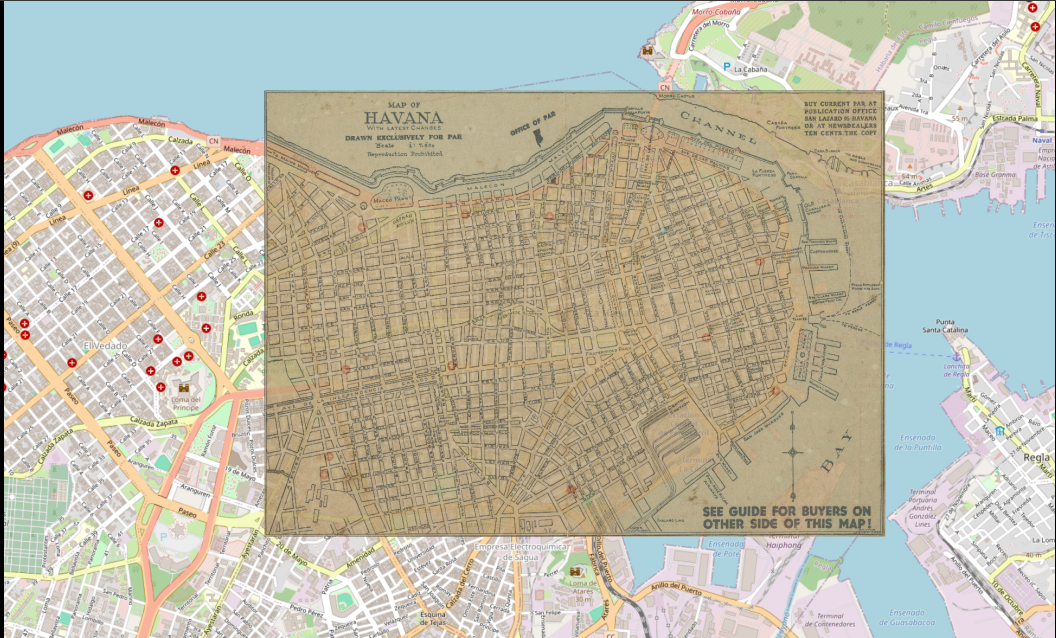
\includegraphics[width=0.5\textwidth]{assets/mapa_superpuesto.png}
    \caption{Mapa superpuesto.}
    \label{fig:poligonos_atipicos}
\end{figure}

\rule{\linewidth}{0.5pt}
\section{Conclusiones}

En este trabajo se ha presentado un m\'etodo automatizado para la digitalizaci\'on y modernizaci\'on de mapas hist\'oricos, con un enfoque particular en la ciudad de La Habana. Se han integrado diversas t\'ecnicas de visi\'on por computadora y aprendizaje profundo para abordar cada fase del procesamiento de mapas, desde la eliminaci\'on de etiquetas textuales hasta la georreferenciaci\'on final.

Los principales logros de esta investigaci\'on incluyen:

\begin{itemize}
    \item \textbf{Preprocesamiento Eficiente:} Se implementaron t\'ecnicas avanzadas para mejorar la calidad de las im\'agenes hist\'oricas, reduciendo ruido y eliminando etiquetas textuales mediante el uso de PaddleOCR y agrupamiento con K-Means.
    \item \textbf{Generaci\'on de Mapas de Calor con Redes Neuronales Convolucionales:} Se desarroll\'o un modelo basado en CNNs para detectar calles y bloques urbanos en los mapas hist\'oricos, proporcionando informaci\'on clave para la segmentaci\'on de im\'agenes.
    \item \textbf{Segmentaci\'on Precisa con Flood Fill:} Se emple\'o un algoritmo modificado de Flood Fill para identificar componentes conexas en los mapas, permitiendo una mejor extracci\'on de bloques urbanos mediante el uso del heatmap generado.
    \item \textbf{Vectorizaci\'on y Simplificaci\'on de Pol\'igonos:} Se aplicaron t\'ecnicas de vectorizaci\'on utilizando GDAL y simplificaci\'on mediante los algoritmos de Ramer-Douglas-Peucker y Shapely, optimizando la representaci\'on geom\'etrica de los bloques urbanos.
    \item \textbf{Identificaci\'on de Pol\'igonos At\'ipicos mediante DBSCAN:} Se implement\'o un modelo de detecci\'on de outliers utilizando DBSCAN, con hiperpar\'ametros optimizados mediante optimizaci\'on bayesiana, logrando una mejor detecci\'on de estructuras urbanas inusuales.
    \item \textbf{Matching de Outliers para Georreferenciaci\'on:} Se estableci\'o un procedimiento basado en normalizaci\'on, an\'alisis topol\'ogico y comparaci\'on con el \'{\i}ndice de Jaccard para asociar estructuras en mapas hist\'oricos con sus equivalentes en mapas modernos.
    \item \textbf{Superposici\'on Geoespacial de Mapas:} Finalmente, se realiz\'o la georreferenciaci\'on de los mapas hist\'oricos mediante homograf\'ia y superposici\'on en sistemas de informaci\'on geogr\'afica, permitiendo su integraci\'on con herramientas modernas de an\'alisis geoespacial.
\end{itemize}

\subsection{Limitaciones y Trabajo Futuro}

A pesar de los avances logrados, el m\'etodo propuesto presenta algunas limitaciones, entre ellas:

\begin{itemize}
    \item La calidad de los resultados depende en gran medida del estado de los mapas hist\'oricos originales. Mapas con degradaci\'on severa o detalles borrosos pueden afectar la precisi\'on del proceso.
    \item El modelo de clasificaci\'on basado en CNN podr\'ia beneficiarse de un dataset m\'as extenso y variado para mejorar su capacidad de generalizaci\'on.
    \item La georreferenciaci\'on se basa en la identificaci\'on de outliers urbanos, lo que puede no ser suficiente en algunos casos con mapas muy homog\'eneos.
\end{itemize}

Como trabajo futuro, se propone mejorar el modelo de clasificaci\'on de calles incorporando t\'ecnicas de aprendizaje semi-supervisado y aumentar la precisi\'on de la georreferenciaci\'on mediante la integraci\'on con datos complementarios, como im\'agenes satelitales y registros cartogr\'aficos adicionales.




\renewcommand\refname{Referencias}

\begin{thebibliography}{}

  \sloppypar
  \bibitem{area} Arteaga Moreno, F. J. (2009). Cálculo del área de un polígono simple: una demostración personal. Lección inaugural, septiembre de 2009.


  \bibitem{ocr} Du, Y., Li, C., Guo, R., Yin, X., Liu, W., Zhou, J., ... \& Wang, H. (2020). Pp-ocr: A practical ultra lightweight ocr system. arXiv preprint arXiv:2009.09941. 

    \bibitem{mobilenet} Koonce, B., \& Koonce, B. (2021). MobileNetV3. Convolutional Neural Networks with Swift for Tensorflow: Image Recognition and Dataset Categorization, 125-144.

    \bibitem{diffbin} Liao, M., Zou, Z., Wan, Z., Yao, C., \& Bai, X. (2022). Real-time scene text detection with differentiable binarization and adaptive scale fusion. IEEE transactions on pattern analysis and machine intelligence, 45(1), 919-931.

    \bibitem{rdp} Ehret, U., \& Neuper, M. (2014, May). Applying the Ramer-Douglas-Peucker algorithm to compress and characterize time-series and spatial fields of precipitation. In EGU General Assembly Conference Abstracts (p. 13537).

    \bibitem{shapely} Gillies, S. (2013). The shapely user manual. URL https://pypi. org/project/Shapely.

    \bibitem{floodfill} Shuaeb, S. M., Kamruzzaman, M., \& Ali, M. H. (2021). Extracting a bounded region from a map using flood fill algorithm. Asian Journal of Research in Computer Science, 7(1), 14-20.

    \bibitem{qgis} Moyroud, N., \& Portet, F. (2018). Introduction to QGIS. QGIS and generic tools, 1, 1-17.

    \bibitem{shoelace} Lee, Y., \& Lim, W. (2017). Shoelace formula: Connecting the area of a polygon and the vector cross product. The Mathematics Teacher, 110(8), 631-636.

    \bibitem{osm} Map, O. S. (2017). Open street map. Acessado em, 12.

    \bibitem{jaccard} Leydesdorff, L. (2008). On the normalization and visualization of author co‐citation data: Salton's Cosine versus the Jaccard index. Journal of the American Society for Information Science and Technology, 59(1), 77-85.
    
    \bibitem{auc} Marzban, C. (2004). The ROC curve and the area under it as performance measures. Weather and Forecasting, 19(6), 1106-1114.

    \bibitem{brier} Rufibach, K. (2010). Use of Brier score to assess binary predictions. Journal of clinical epidemiology, 63(8), 938-939.

    \bibitem{precission} Arora, M., Kanjilal, U., \& Varshney, D. (2016). Evaluation of information retrieval: precision and recall. International Journal of Indian Culture and Business Management, 12(2), 224-236.

    \bibitem{dice} Bertels, J., Eelbode, T., Berman, M., Vandermeulen, D., Maes, F., Bisschops, R., \& Blaschko, M. B. (2019). Optimizing the dice score and jaccard index for medical image segmentation: Theory and practice. In Medical Image Computing and Computer Assisted Intervention–MICCAI 2019: 22nd International Conference, Shenzhen, China, October 13–17, 2019, Proceedings, Part II 22 (pp. 92-100). Springer International Publishing.

    \bibitem{iou} Cheng, B., Girshick, R., Dollár, P., Berg, A. C., \& Kirillov, A. (2021). Boundary IoU: Improving object-centric image segmentation evaluation. In Proceedings of the IEEE/CVF conference on computer vision and pattern recognition (pp. 15334-15342).
\end{thebibliography}

\newpage

\section{Anexos}

\begin{table*}[ht]
\centering
\caption{ROC\_AUC (Normal)}
\label{tab:roc_auc_normal}
\setlength{\tabcolsep}{6pt} % Ajusta el espacio entre columnas
\renewcommand{\arraystretch}{1.2} % Ajusta la altura de las filas
\begin{tabular}{|l|l|l|l|}
\hline
model & Modelo Anotado Manualmente & Modelo Semi-Aleatorio & Modelo Sintético \\ \hline
ohcah\_cpcu\_000013375.jpg & 0.3309 & 0.1623 & \textbf{0.5031} \\ \hline
ohcah\_cpcu\_000013376.jpg & 0.3208 & 0.2189 & \textbf{0.5000} \\ \hline
ohcah\_cpcu\_000013380.jpg & \textbf{0.5990} & 0.1516 & 0.4983 \\ \hline
ohcah\_cpcu\_000013393.jpg & \textbf{0.5473} & 0.2940 & 0.5006 \\ \hline
ohcah\_cpcu\_000013400.jpg & \textbf{0.6038} & 0.2762 & 0.5017 \\ \hline
ohcah\_cpcu\_000013433.jpg & \textbf{0.6459} & 0.2624 & 0.5027 \\ \hline
\end{tabular}
\end{table*}



\begin{table*}[ht]
\centering
\caption{ROC\_AUC (Labeless)}
\label{tab:roc_auc_labeless}
\setlength{\tabcolsep}{6pt}
\renewcommand{\arraystretch}{1.2}
\begin{tabular}{|l|l|l|l|}
\hline
model & Modelo Anotado Manualmente & Modelo Semi-Aleatorio & Modelo Sintético \\ \hline
ohcah\_cpcu\_000013375.jpg & 0.3559 & 0.1678 & \textbf{0.5031} \\ \hline
ohcah\_cpcu\_000013376.jpg & 0.3038 & 0.2129 & \textbf{0.4999} \\ \hline
ohcah\_cpcu\_000013380.jpg & \textbf{0.6156} & 0.1610 & 0.4983 \\ \hline
ohcah\_cpcu\_000013393.jpg & \textbf{0.5434} & 0.2671 & 0.5006 \\ \hline
ohcah\_cpcu\_000013400.jpg & \textbf{0.6072} & 0.2788 & 0.5017 \\ \hline
ohcah\_cpcu\_000013433.jpg & \textbf{0.6914} & 0.2837 & 0.5027 \\ \hline
\end{tabular}
\end{table*}



\begin{table*}[ht]
\centering
\caption{Average\_Precision (Normal)}
\label{tab:avg_prec_normal}
\setlength{\tabcolsep}{6pt}
\renewcommand{\arraystretch}{1.2}
\begin{tabular}{|l|l|l|l|}
\hline
model & Modelo Anotado Manualmente & Modelo Semi-Aleatorio & Modelo Sintético \\ \hline
ohcah\_cpcu\_000013375.jpg & 0.0330 & 0.0276 & \textbf{0.0490} \\ \hline
ohcah\_cpcu\_000013376.jpg & 0.0506 & 0.0455 & \textbf{0.0755} \\ \hline
ohcah\_cpcu\_000013380.jpg & \textbf{0.0355} & 0.0171 & 0.0307 \\ \hline
ohcah\_cpcu\_000013393.jpg & \textbf{0.1552} & 0.0879 & 0.1333 \\ \hline
ohcah\_cpcu\_000013400.jpg & \textbf{0.3625} & 0.1774 & 0.2608 \\ \hline
ohcah\_cpcu\_000013433.jpg & \textbf{0.3056} & 0.1341 & 0.2052 \\ \hline
\end{tabular}
\end{table*}



\begin{table*}[ht]
\centering
\caption{Average\_Precision (Labeless)}
\label{tab:avg_prec_labeless}
\setlength{\tabcolsep}{6pt}
\renewcommand{\arraystretch}{1.2}
\begin{tabular}{|l|l|l|l|}
\hline
model & Modelo Anotado Manualmente & Modelo Semi-Aleatorio & Modelo Sintético \\ \hline
ohcah\_cpcu\_000013375.jpg & 0.0341 & 0.0276 & \textbf{0.0490} \\ \hline
ohcah\_cpcu\_000013376.jpg & 0.0494 & 0.0449 & \textbf{0.0755} \\ \hline
ohcah\_cpcu\_000013380.jpg & \textbf{0.0372} & 0.0172 & 0.0307 \\ \hline
ohcah\_cpcu\_000013393.jpg & \textbf{0.1537} & 0.0852 & 0.1333 \\ \hline
ohcah\_cpcu\_000013400.jpg & \textbf{0.3622} & 0.1784 & 0.2608 \\ \hline
ohcah\_cpcu\_000013433.jpg & \textbf{0.3557} & 0.1367 & 0.2052 \\ \hline
\end{tabular}
\end{table*}



\begin{table*}[ht]
\centering
\caption{Brier\_Score (Normal)}
\label{tab:brier_score_normal}
\setlength{\tabcolsep}{6pt}
\renewcommand{\arraystretch}{1.2}
\begin{tabular}{|l|l|l|l|}
\hline
model & Modelo Anotado Manualmente & Modelo Semi-Aleatorio & Modelo Sintético \\ \hline
ohcah\_cpcu\_000013375.jpg & \textbf{0.4433} & 0.6465 & 0.9453 \\ \hline
ohcah\_cpcu\_000013376.jpg & \textbf{0.3243} & 0.4682 & 0.9202 \\ \hline
ohcah\_cpcu\_000013380.jpg & \textbf{0.1696} & 0.6956 & 0.9672 \\ \hline
ohcah\_cpcu\_000013393.jpg & \textbf{0.1256} & 0.4480 & 0.8647 \\ \hline
ohcah\_cpcu\_000013400.jpg & \textbf{0.2538} & 0.5782 & 0.7360 \\ \hline
ohcah\_cpcu\_000013433.jpg & \textbf{0.1671} & 0.6098 & 0.7909 \\ \hline
\end{tabular}
\end{table*}



\begin{table*}[ht]
\centering
\caption{Brier\_Score (Labeless)}
\label{tab:brier_score_labeless}
\setlength{\tabcolsep}{6pt}
\renewcommand{\arraystretch}{1.2}
\begin{tabular}{|l|l|l|l|}
\hline
model & Modelo Anotado Manualmente & Modelo Semi-Aleatorio & Modelo Sintético \\ \hline
ohcah\_cpcu\_000013375.jpg & \textbf{0.4713} & 0.6959 & 0.9453 \\ \hline
ohcah\_cpcu\_000013376.jpg & \textbf{0.3713} & 0.5305 & 0.9202 \\ \hline
ohcah\_cpcu\_000013380.jpg & \textbf{0.1764} & 0.7434 & 0.9672 \\ \hline
ohcah\_cpcu\_000013393.jpg & \textbf{0.1269} & 0.5358 & 0.8647 \\ \hline
ohcah\_cpcu\_000013400.jpg & \textbf{0.2544} & 0.5836 & 0.7360 \\ \hline
ohcah\_cpcu\_000013433.jpg & \textbf{0.1595} & 0.6262 & 0.7909 \\ \hline
\end{tabular}
\end{table*}
    
    

\end{document}